\section*{Question 7}
\textit{Using the information that the window length necessary to calculate the energy spectrum should be at least 50 integral time scales, calculate the energy spectra for both datasets.}

\begin{figure}[ht]
\centering
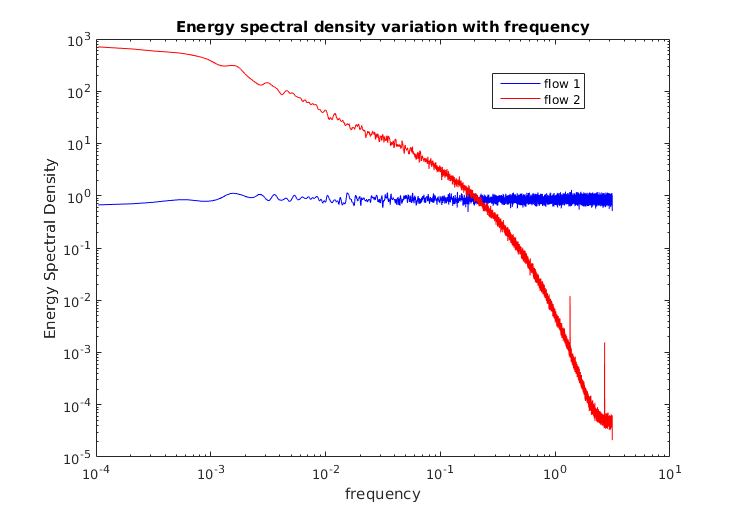
\includegraphics[scale=0.7]{./TEXT/esd.png}
\caption{Comparison between the energy spectral densities of both flow cases as they change with frequency for a window size of $20'000$ data points}
\label{esd}
\end{figure}

Figure \ref{esd} shows how the spectral energy varies with frequency. Flow 2 exhibits high energy for low frequencies of the order of $10^{3}$, whereas flow 1 has a constant energy of order $1$ for all frequencies.